%#################################################################
\chapter{Proposta de DSL}\label{propostaDSL}
%#################################################################

Este capítulo apresenta a proposta central deste trabalho. 
A Seção \ref{sec:reqDSL} aponta os requisitos levantados para a construção da \ac{DSL}. 
A Seção \ref{sec:decDSL} descreve as decisões de projeto referente aos requisitos. 
A arquitetura da implementação da proposta é detalhada na Seção \ref{sec:arqDSL}. 
A demonstração do protótipo construído ocorre na Seção \ref{sec:protDSL} e, por fim, as lições do capítulo são pontuadas na Seção \ref{sec:licDSL}.

%#################################################################
\section{Requisitos da Linguagem} \label{sec:reqDSL}
%#################################################################

Esta seção lista os requisitos que foram definidos com base na literatura utilizada neste trabalho, bem como no conhecimento prévio dos pesquisadores envolvidos na condução do estudo. 
Estes requisitos são relacionados diretamente com as decisões de projeto.

\begin{itemize}

\item\textit{\textbf{RQ1. A \ac{DSL} precisa ser disponibilizada sob uma licença open source.}} 
Como o foco da proposta é no processo de ensino é fundamental que a linguagem seja de código aberto. 
A vantagem que este requisito proporciona é a posterior evolução e manutenção colaborativa com o envolvimento de outros desenvolvedores.

\item\textit{\textbf{RQ2. A \ac{DSL} deve permitir representar textualmente modelos conceituais de \acp{BD}.}} 
Como é um objetivo que a solução seja outra opção em relação as abordagens gráficas, esse requisito se justifica. 
Isso permite o foco na compreensão do domínio e no desenvolvimento da \ac{DSL}.

\item\textit{\textbf{RQ3. Os modelos conceituais devem dar suporte a definição de entidades, atributos, relações e cardinalidades.}} 
As ferramentas utilizadas para o desenvolvimento da linguagem precisam permitir que sejam implementados os conceitos de domínio que regem a estrutura de \ac{DER} tradicional.

\item\textit{\textbf{RQ4. Os modelos conceituais devem dar suporte a definição de atributos identificadores, generalização/especialização, auto-relacionamentos e relacionamentos ternários.}} 
A linguagem deve permitir que conceitos mais sofisticados dos domínios sejam definidos.

\item\textit{\textbf{RQ5. A implementação da \ac{DSL} deve realizar a transformação do modelo conceitual para o lógico.}} 
A solução deve realizar a transformação do conceitual para o lógico, exibindo o resultado gerado ao usuário.

\item\textit{\textbf{RQ6. A implementação da \ac{DSL} deve gerar modelos físicos equivalentes, com base no modelo conceitual ou lógico.}} 
A solução precisa realizar a geração de instruções \ac{SQL} para diferentes \acp{SGBD}.

\end{itemize}

%#################################################################
\section{Decisões de Projeto} \label{sec:decDSL}
%#################################################################

Nesta seção são descritas as decisões de projeto para criar a \ac{DSL} textual que suporte todos os requisitos discutidos na Seção \ref{sec:reqDSL}. 
Para cada decisão de projeto são indicados os seus requisitos associados.

\begin{itemize}
    \item\textit{\textbf{DP1. A solução deve adotar um \ac{LW} open source no auxílio da implementação da \ac{DSL} textual (RQ1, RQ2).}} 
    Mediante a investigação conduzida durante este estudo foi selecionado o \ac{LW} Xtext para o desenvolvimento da proposta por ser um \textit{framework open source} focado no desenvolvimento de \acp{DSL} textuais, fornecendo toda a infraestrutura necessária. 
    Além disto, o Xtext é uma ferramenta com alto nível de maturidade, documentação detalhada e uma comunidade ativa. 
    
    \item\textit{\textbf{DP2. A \ac{DSL} deve fornecer uma representação textual que seja equivalente ao modelo \ac{ER} gráfico usualmente utilizado (RQ3, RQ4).}} 
    Para os requisitos cobertos por esta decisão de projeto foi adotada a estratégia de se realizar uma análise nas ferramentas averiguadas no mapeamento descrito no \autoref{mapeamentoLiteratura}, bem como no livro referência de \citeonline{Heuser:2009}.
    
    \item\textit{\textbf{DP3. A solução deve realizar a transformação entre os modelos (RQ5).}} 
    O Xtext usa modelos do \ac{EMF} como a representação na memória de qualquer arquivo de texto analisado. 
    Esse grafo de objetos na memória é chamado de árvore sintática abstrata, do inglês \ac{AST}. 
    Esses conceitos também são chamados de gráficos de objeto de documento, do inglês \ac{DOM}, modelo semântico ou simplesmente modelo. 
    Desta forma, existe a representação do modelo da gramática na forma de um metamodelo central no núcleo do \ac{EMF}, chamado de modelo \textit{Ecore}. 
    Tendo o \textit{Ecore} da \ac{DSL} proposta como uma representação, é possível então aplicar regras de transformação, gerando assim outros modelos.
    
    \item\textit{\textbf{DP4. A solução deve prover a integração entre a \ac{DSL} e outras tecnologias (RQ6).}} 
    A solução deve permitir a realização da exportação dos modelos construídos para um formato de instruções \ac{SQL}, representando assim o modelo físico. 
    Inicialmente, essa integração será realizada para o SQL Server, o MySQL e o PostgreSQL. 
    Foram estabelecidas essas tecnologias pois são alguns dos \acp{SGBD} mais utilizados no mercado, conforme foi descrito nos tópicos da \autoref{ssec:SGBDRelacionais}.
\end{itemize}


%#################################################################
\section{Arquitetura} \label{sec:arqDSL}
%#################################################################

O \textit{framework} Xtext gera toda a infraestrutura para a criação de linguagens com base fundamentalmente nas gramáticas definidas. 
A \autoref{fig:arqXtext} fornece uma visão geral em um nível abstrato da arquitetura do Xtext. 
% Tendo esse contexto estabelecido, começou-se a definição da \ac{DSL}. 

\begin{figure}[!htb]
    \centering
    \caption{Arquitetura geral do Xtext.}
    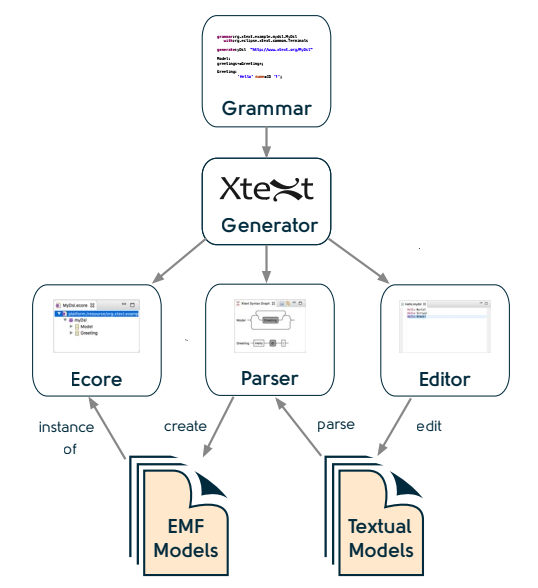
\includegraphics[width=0.6\textwidth]{img/ArquiteturaXtext.jpg}
    \label{fig:arqXtext}
    \fonte{\citeonline{XtextSirius:2017}.}
\end{figure}

Foram implementadas duas versões da gramática no protótipo da \ac{DSL}. 
A seguir as arquiteturas dessas implementações são descritas e pontua-se as diferenças entre elas. 
Essa abordagem foi definida tendo em vista que será realizada uma avaliação preliminar junto a um grupo focal. 
A partir dos resultados dessa avaliação, objetiva-se gerar uma versão final da gramática e, consequentemente, da arquitetura.

\begin{figure}[!htb]
    \centering
    \caption{Representação do modelo \textit{Ecore} da 1º versão da DSL.}
    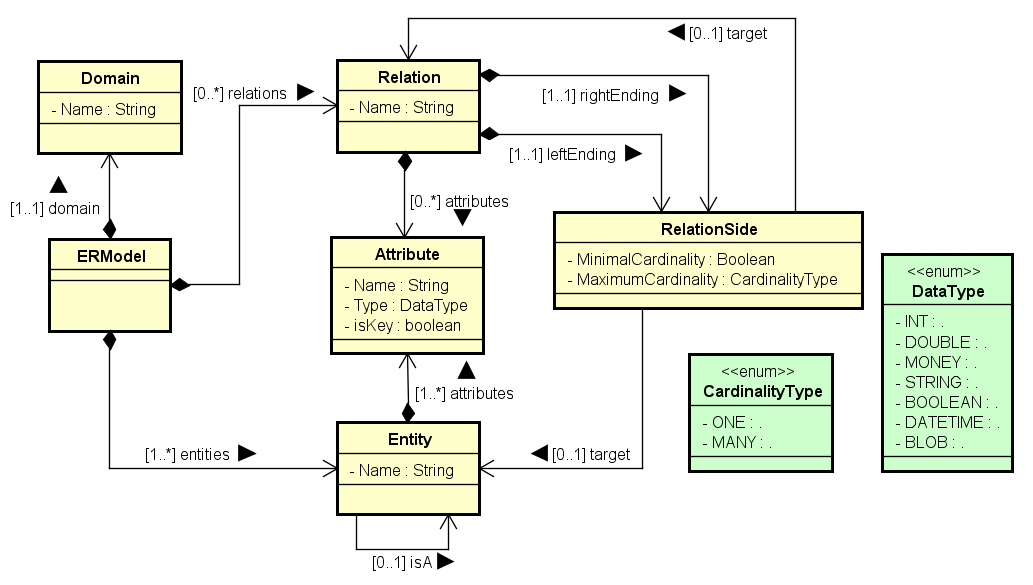
\includegraphics[width=1\textwidth]{img/erDslClassDiagram.png}
    \fonte{O autor.}
    \label{fig:ERDSL}
\end{figure}

A \autoref{fig:ERDSL} mostra um diagrama de classes para representar o modelo \textit{Ecore} da primeira versão criada para esta proposta. 
O elemento central do modelo é a classe \texttt{ERModel}, a qual corresponde por uma composição com outros elementos. 
O \texttt{ERModel} deve possuir um \texttt{Domain} associado, simbolizando o nome da base de dados modelada. 

Um \texttt{ERModel} também deve conter um ou mais elementos \texttt{Entity}. 
Um elemento \texttt{Entity} pode se relacionar com outro elemento \texttt{Entity}, cobrindo assim o conceito de generalização/especialização. 
Um \texttt{Entity} é também uma composição de uma ou mais classes \texttt{Attribute}. 
Definiu-se os tipos de dados em uma lista enumerada no elemento \texttt{DataType}.

Em seguida, um \texttt{ERModel} pode ser composto de uma ou mais relações, retratado como a classe \texttt{Relation}. 
Uma \texttt{Relation} por sua vez é formada por duas classes \texttt{RelationSide}, os quais são as cardinalidades da esquerda e da direita em uma relação. 
Estas duas relações possuem uma referência chamada \texttt{Target}, que pode ser uma \texttt{Entity} ou uma \texttt{Relation}. 
A inclusão da possibilidade de se referenciar uma \texttt{Relation} se faz necessário para cobrir a modelagem dos relacionamentos ternários.

Finalmente, tem-se o conceito das cardinalidades. 
Nele as cardinalidades possíveis, mantidas em atributos da \texttt{RelationSide}, são os tipos enumerados em \texttt{CardinalityType}, sendo \texttt{One} para um e \texttt{Many} para muitos. 
Por meio das regras da gramática garante-se que a cardinalidade mínima é implícita, tendo a palavra reservada \textit{zero} para simbolizar quando uma cardinalidade mínima pode ser nula. 
Isto significa que, em uma modelagem onde uma cardinalidade mínima \textit{zero} é omitida, assume-se que ela automaticamente é igual a um.

% \begin{figure} [!htb]
%     \centering
%     \caption{Representação do modelo ECORE da segunda versão da DSL.}
%     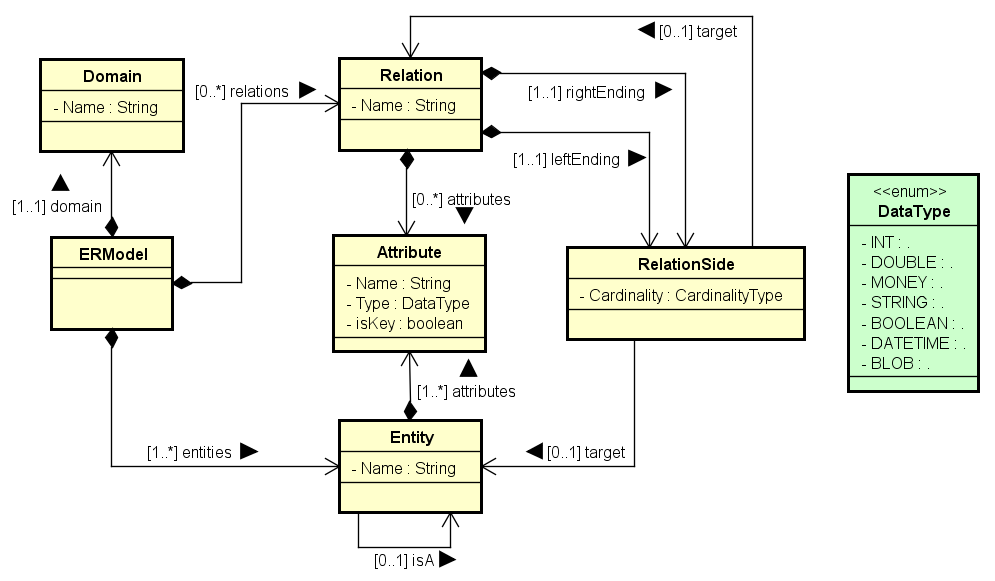
\includegraphics[width=0.8\textwidth]{img/erDsl2ClassDiagram.png}
%     \fonte{O autor.}
%     \label{fig:ERDSL2}
% \end{figure}

Estruturalmente o modelo \textit{Ecore} da segunda versão \ac{DSL} não muda significativamente.%, como pode-se observar na Figura \ref{fig:ERDSL2}. 
A única diferença com maior impacto é a opção pela definição da cardinalidade utilizando-se as quatro combinações possíveis como termos reservados, armazenados diretamente no atributo \texttt{Cardinality} de \texttt{RelationSide}.

%#################################################################
\section{Protótipo} \label{sec:protDSL}
%#################################################################
\definecolor{javared}{rgb}{0.6,0,0} % for strings
\definecolor{javagreen}{rgb}{0.25,0.5,0.35} % comments
\definecolor{javapurple}{rgb}{0.5,0,0.35} % keywords
\definecolor{javadocblue}{rgb}{0.25,0.35,0.75} % javadoc
\definecolor{verde}{rgb}{0.25,0.5,0.35}
\definecolor{jpurple}{rgb}{0.5,0,0.35}
\definecolor{darkgreen}{rgb}{0.0, 0.2, 0.13}


\lstdefinelanguage{Xtext}{
  sensitive = true,
  keywords={},
  keywords=[2]{ERModel, Domain, Attribute, Entity, Relation, RelationSide, DataType, CardinalityType},
  keywords=[3]{grammar, with, generate, Terminals, enum},
  otherkeywords={*, ?, +, *=, ?=, +=, |},
  keywordstyle=\color{black}\bfseries,
  keywordstyle=[2]\color{javadocblue}\bfseries,
  keywordstyle=[3]\color{javapurple}\bfseries,% for example
%   backgroundcolor=\color{cyan!10},
%   numbers=left,
%   stepnumber=1,
  numbersep=8pt,
  showstringspaces=false,
  breaklines=true,
  frame=top,
  comment=[l]{//},
  morecomment=[s]{/*}{*/},
  commentstyle=\color{black}\ttfamily,
  stringstyle=\color{javared}\ttfamily,
  morestring=[b]',
  morestring=[b]"
  }
  
  \lstdefinelanguage{ERDSL}{
  sensitive = true,
  keywords={},
  keywords=[2]{Domain, Entities, Relationships, isIdentifier, isRelatedWith, isA, zero, one, many},
  keywords=[3]{int, money, string, datetime, file},
  otherkeywords={*, ?, +, *=, ?=, +=, |},
  keywordstyle=\color{black}\bfseries,
  keywordstyle=[2]\color{javapurple}\bfseries,
  keywordstyle=[3]\color{javadocblue}\bfseries,% for example
%   backgroundcolor=\color{cyan!10},
%   numbers=left,
%   stepnumber=1,
  captionpos=t,
  numbersep=8pt,
  showstringspaces=false,
  breaklines=true,
  frame=top,
  comment=[l]{//},
  morecomment=[s]{/*}{*/},
  commentstyle=\color{black}\ttfamily,
  stringstyle=\color{javared}\ttfamily,
  morestring=[b]',
  morestring=[b]"
  }



Na fase atual do trabalho a linguagem a nível conceitual não se encontra totalmente finalizada. 
Existem tópicos relativos a validação de escopo, como no caso do tratamento de referências cruzadas indesejadas, e outras restrições inerentes ao modelo \ac{ER} que devem ser analisadas e então implementadas. 
A definição da \ac{DSL} criada é exibida na \autoref{fig:DSLvs1}.

\begin{figure}
    \centering
    \caption{Implementação da 1º versão da DSL.}
    \label{fig:DSLvs1}
    \begin{scriptsize}
    \begin{lstlisting}[language = Xtext , frame = trbl]
grammar org.xtext.unipampa.lesse.erdsl with org.eclipse.xtext.common.Terminals

generate erdsl "http://www.xtext.org/unipampa/lesse/erdsl/"

ERModel:
	domain=Domain ";"
	("Entities{") entities+=Entity+ ("};")
	("Relationships{") relations+=Relation* ("};");

Domain:
	"Domain" name=ID;

Entity:
	name=ID ("isA" isA+=[Entity])* 
	("{" attributes+=Attribute ("," attributes+=Attribute)* "}")?;

Attribute:
  name=ID ":" type=DataType (isKey?="isIdentifier")?;

Relation:
	(name=ID)? 
	("[" leftEnding=RelationSide 
	"isRelatedWith" 
	rightEnding=RelationSide "]")
	("{" attributes+=Attribute 
	("," attributes+=Attribute)* "}")*;
	
RelationSide:
	((minimalCardinality?="zero")?)	maximumCardinality=CardinalityType	
	target=[Entity] | target=[Relation];

enum DataType:
	INT="int" | DOUBLE="double" | MONEY="money" | STRING="string" | 
	BOOLEAN="boolean" | DATETIME="datetime" | BLOB="file";

enum CardinalityType:
	One="one" | Many="many";
    \end{lstlisting}
    \end{scriptsize}    
    \fonte{O autor.}
\end{figure}


O comando \texttt{grammar} especifica o nome da \ac{DSL}, enquanto que a instrução \texttt{with} declara uma herança de outra linguagem. 
No caso da gramática proposta, será utilizado uma gramática padrão do Xtext, chamada \texttt{Terminals}, a qual fornece algumas regras predefinidas como, por exemplo, a regra \texttt{ID} para identificadores ou \texttt{INT} para inteiros. 
O comando \texttt{generate} é a instrução que produz a \ac{AST} da linguagem.

A primeira regra, chamada de regra de entrada, define como é a estrutura geral da linguagem. 
Palavras e símbolos entre aspas duplas ou simples indicam as palavras reservadas. 
Por exemplo, o objeto \texttt{Entities} é obrigatoriamente precedido de "\texttt{Entities\{}". 
Este objeto representa uma espécie de \textit{container}, sendo isto indicado por meio do operador de atribuição \texttt{+=}. 
Ele é um objeto que pode conter outros objetos, no caso um ou mais \texttt{Entity} (entidades). 
É estabelecido que cada arquivo da \ac{DSL} deve também ser composto de um \texttt{Domain} (domínio) e zero ou mais \texttt{Relation} (relações). 

Para melhor entendimento, deve-se deixar claro que a multiplicidade é indicada por \texttt{*} (zero ou muitos), \texttt{+} (um ou muitos) ou \texttt{?} (zero ou um). 
Ao não se colocar nenhum desses operadores, implicitamente se espera então apenas uma ocorrência. 
Em relação as atribuições, quando apenas um \texttt{=} for especificado significa que o objeto da esquerda espera apenas um registro. 
Logo, para \texttt{+=} espera-se então zero, uma ou mais ocorrências. 

O objeto \texttt{Domain} é precedido de uma palavra reservada com o mesmo nome, seguido de um identificador. 
A entidade é definida pela palavra \texttt{Entity} e um nome identificador específico para este objeto. 
A definição de uma herança é opcional por meio da palavra reservada \texttt{isA}. 
Após a definição do nome, abre-se um corpo de chaves em que são especificados os atributos da entidade. 
Uma entidade deve conter ao menos um atributo, mas ele não precisa ser identificador por conta da possível existência de entidades fracas. 

As regras compostas só são realizadas devido a possibilidade de se agrupar expressões com o uso de parênteses, além da possibilidade de se utilizar outras regras por meio de referências cruzadas. 
Os colchetes entre a regra \texttt{Entity} servem para indicar que se almeja usar apenas o atributo \texttt{name} que identifica o objeto. 
% Se esse detalhe não for especificado então o compilador da linguagem interpretaria que é necessário aplicar toda a regra \texttt{Entity} novamente, ou seja, se iniciaria a definição de outra entidade entrando assim em um \textit{loop}. 
Os atributos das entidades são definidos por um nome, herdando a regra \texttt{ID} de \texttt{Terminals}, e atributos \texttt{isIdentifier} opcionais para simbolizar chaves primárias. 

A relação é definida, já dentro do corpo do bloco \texttt{Relationships}, com uma declaração opcional de sua identificação. 
Em seguida, são abertos colchetes e deve-se especificar dois elementos \texttt{RelationSide} como referência aos atributos \texttt{leftEnding} e \texttt{rightEnding}. 
Estes atributos representam os lados de uma relação. 
Estes objetos devem ser separados pela expressão \texttt{isRelatedWith}. 
Os lados da relação são definidos na regra \textit{RelationSide}, composta de dois atributos. 
O atributo \texttt{minimalCardinality} é opcional, indicado pelo operador \texttt{?}, e aceita apenas a palavra reservada \texttt{zero}. 
O atributo \texttt{maximumCardinality} aceita um objeto \texttt{CardinalityType}.

Os tipos de atributo estão contidos em uma lista enumerada chamada \texttt{DataType}, na esquerda fica a representação no modelo \textit{Ecore}. 
Na direita está a palavra reservada que é usada na linguagem. 
O símbolo condicional \texttt{|} significa o operador lógico \textit{OR} (ou) e serve para separar cada definição \texttt{<chave> = <valor>} como uma opção dentro da lista. 
Das três cardinalidades possíveis, duas estão definidas em outra lista enumerada chamada \texttt{CardinalityType}. 
Na \autoref{fig:DSLvs2} exibe a principal mudança entre as versões da \ac{DSL} proposta, a qual diz respeito a cardinalidade explícita. 
A \autoref{fig:ERDSLSyntax} e a \autoref{fig:ERDSL2Syntax} apresentam uma representação gráfica das sintaxes de ambas as gramáticas.

\begin{figure}[!htb]
    \centering
    \caption{Fragmento de implementação da 2º versão da DSL.}
    \label{fig:DSLvs2}
    \begin{footnotesize}
\begin{lstlisting}[language = Xtext , frame = trbl]
Relation:
	(name=ID)? ("[" leftEnding=RelationSide "relates" 
	rightEnding=RelationSide "]") ("{"attributes+=Attribute 
	("," attributes+=Attribute)* "}")*;

RelationSide:
	Cardinality=("(0,1)" | "(1,1)" | "(0,N)" | "(1,N)")
	target=[Entity] | target=[Relation];
    \end{lstlisting}
    \end{footnotesize} 
    \fonte{O autor}
\end{figure}

\begin{figure}[!htb]
    \centering
    \caption{Representação da sintaxe da 1º versão da DSL.}
    \label{fig:ERDSLSyntax}
    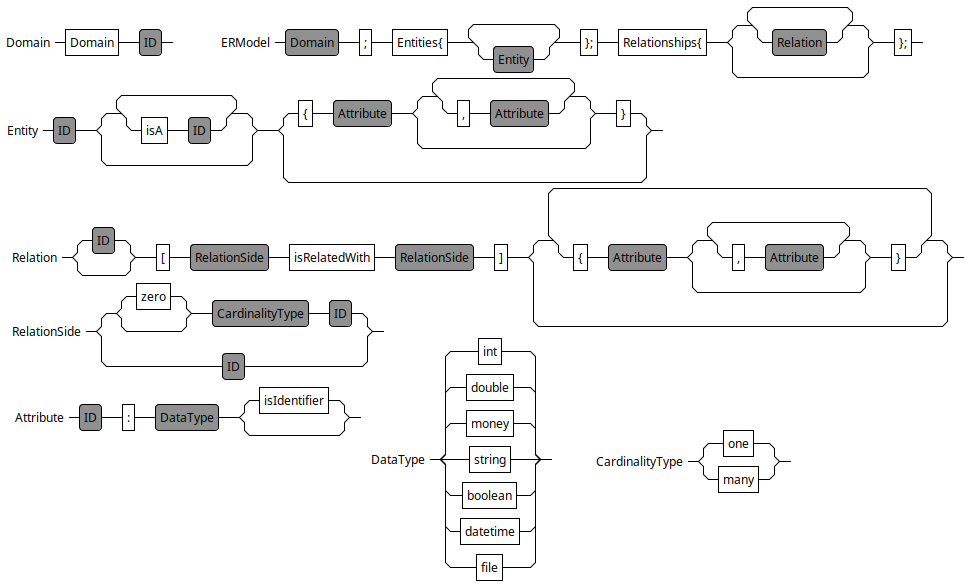
\includegraphics[width=\textwidth]{img/ERDSLSyntaxGraph.png}
    \fonte{O autor.}
\end{figure}

\begin{figure} [!htb]
    \centering
    \caption{Representação da sintaxe da 2º versão da DSL.}
    \label{fig:ERDSL2Syntax}
    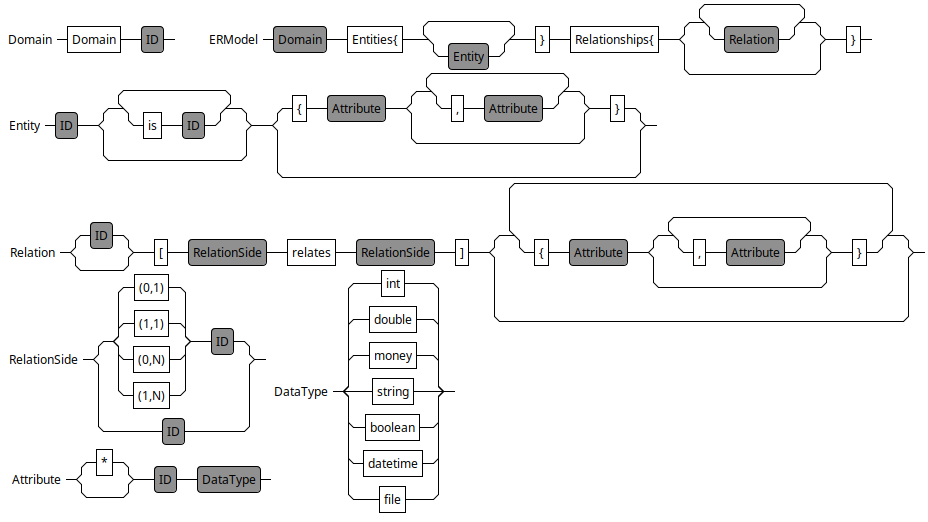
\includegraphics[width=\textwidth]{img/ERDSL2SyntaxGraph.png}
    \fonte{O autor.}
\end{figure}

Na \autoref{fig:DSLvs1Uso} mostra-se um exemplo de uso com um pequeno modelo que aborda uma universidade como domínio. 
Neste protótipo já se pode observar a modelagem de generalização/especialização, auto-relacionamento e relacionamento ternário.

% Para essa transformação existem regras que podem ser aplicadas, sendo que em alguns casos existem inclusive mais de uma opção. 
% Nestes casos estão sendo analisadas a melhores estratégias possíveis, uma vez que durante o processo de transformação será necessário se assumir algumas premissas.

\begin{figure}[!htb]
\centering
\caption{Exemplo de uso da 1º versão da DSL no RCP do Eclipse.}
\label{fig:DSLvs1Uso}
\begin{scriptsize}
\begin{lstlisting}[language = ERDSL, frame = trbl]
Domain University;

Entities{
	Person{ 
		PID: int isIdentifier, 
		Name: string
	}
	Teacher isA Person{ 
		Phone: int,
		Salary:money
	}
	Student isA Person{ 
		Course: string
	} 	
	OutsrcEmployee isA Person{
	    OutsourcedEID: int isIdentifier,
	    Company: string
	}
	Class{
		ClassID: int isIdentifier,
		Course: string,
		Semester: string
	}
	ClassRoom {
		ClassRoomID: int isIdentifier,
		Capacity: int
	}
};

Relationships{	 
	[many Student isRelatedWith many Class]
	TeacherClass [many Teacher isRelatedWith many Class]
	ClassSchedule [many TeacherClass isRelatedWith many ClassRoom]
	        {ClassScheduleID: int, DayOfWeek: datetime, Discipline: string}
	Supervisor [one OutsrcEmployee isRelatedWith many OutsrcEmployee]
};
\end{lstlisting}
\end{scriptsize}
    \fonte{O autor.}
\end{figure}
É importante destacar que neste exemplo são modeladas seis entidades e quatro relacionamentos. 
Contudo, no processo de transformação para o modelo lógico espera-se que seja gerado um esquema textual com mais três entidades, inferindo-se isso através de, por exemplo, relacionamentos \textit{muitos para muitos}. 
Isso ocorreria, nesta amostra, no relacionamento sem identificação, atribuindo automaticamente a nova entidade o nome resultante da concatenação das duas entidades que se relacionam no conceitual. 
Também seriam criadas novas entidades a partir da derivação dos relacionamentos nomeados \texttt{TeacherClass} e \texttt{ClassShedule}, sendo que o último carateriza um relacionamento ternário.
Por fim, o auto-relacionamento \texttt{Supervisor} de \texttt{OutsrcEmployee} implicaria na adição de um novo atributo na entidade no novo modelo.

Com base nos modelos \textit{Ecore} gerados em tempo real, como o gerado a partir do modelo descrito anteriormente e exibido na \autoref{fig:EcoreRealTime}, já está sendo implementada a transformação do modelo conceitual para o lógico. 
A implementação desta transformação está sendo realizada utilizando-se a Xtend, uma \ac{GPL} baseada em Java.

\begin{figure} [!htb]
    \centering
    \caption{Fragmento do modelo \textit{Ecore} gerado em tempo de execução.}
    \label{fig:EcoreRealTime}
    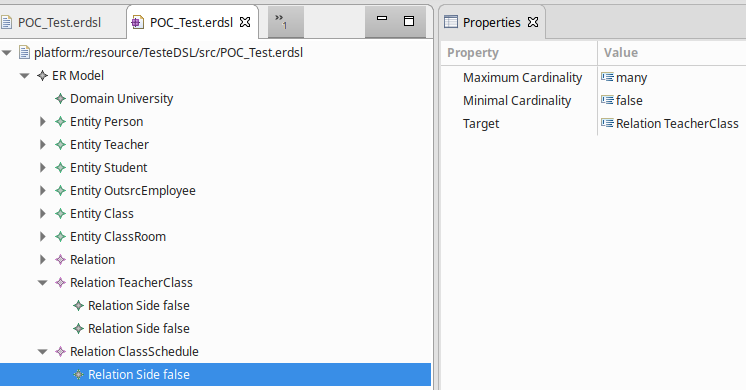
\includegraphics[width=0.65\textwidth]{img/EcoreTempoReal.png}
    \fonte{O autor.}
\end{figure}


%#################################################################
\section{Lições do Capítulo} \label{sec:licDSL}
%#################################################################

Neste capítulo foram expostos os requisitos, as decisões de projeto e a arquitetura da \ac{DSL} proposta. 
Também foi demonstrado como o protótipo da versão preliminar da linguagem foi definido, bem como um exemplo de uso.

Até o momento o Xtext mostrou-se uma \ac{LW} capaz de suprir as necessidades iniciais do projeto, fornecendo suporte completo para a criação de gramáticas com notação \ac{BNF}, uma meta-sintaxe amplamente usada para expressar gramáticas livres de contexto como nas estruturas de linguagens de programação no geral. 
Além de prover a validação da gramática criada, foi gerado um \textit{plugin} tornando assim possível a realização do teste do protótipo em um \ac{RCP} Eclipse. 

%Assim, por meio disso o processo de modelagem com a nova linguagem criada ganhou recursos nativos como formatação, validação com base nas restrições descritas na gramática e \textit{syntax highlighting}. 
%É importante ressaltar que o \textit{plugin} somente pôde ser testado devido a integração nativa fornecida pelo Xtext com o \ac{EMF}, um conjunto de recursos do Eclipse para representar modelos e gerar código equivalente. 